\chapter{Diagramme d'activité}

\section{Diagramme}

\begin{figure}
  \centering
  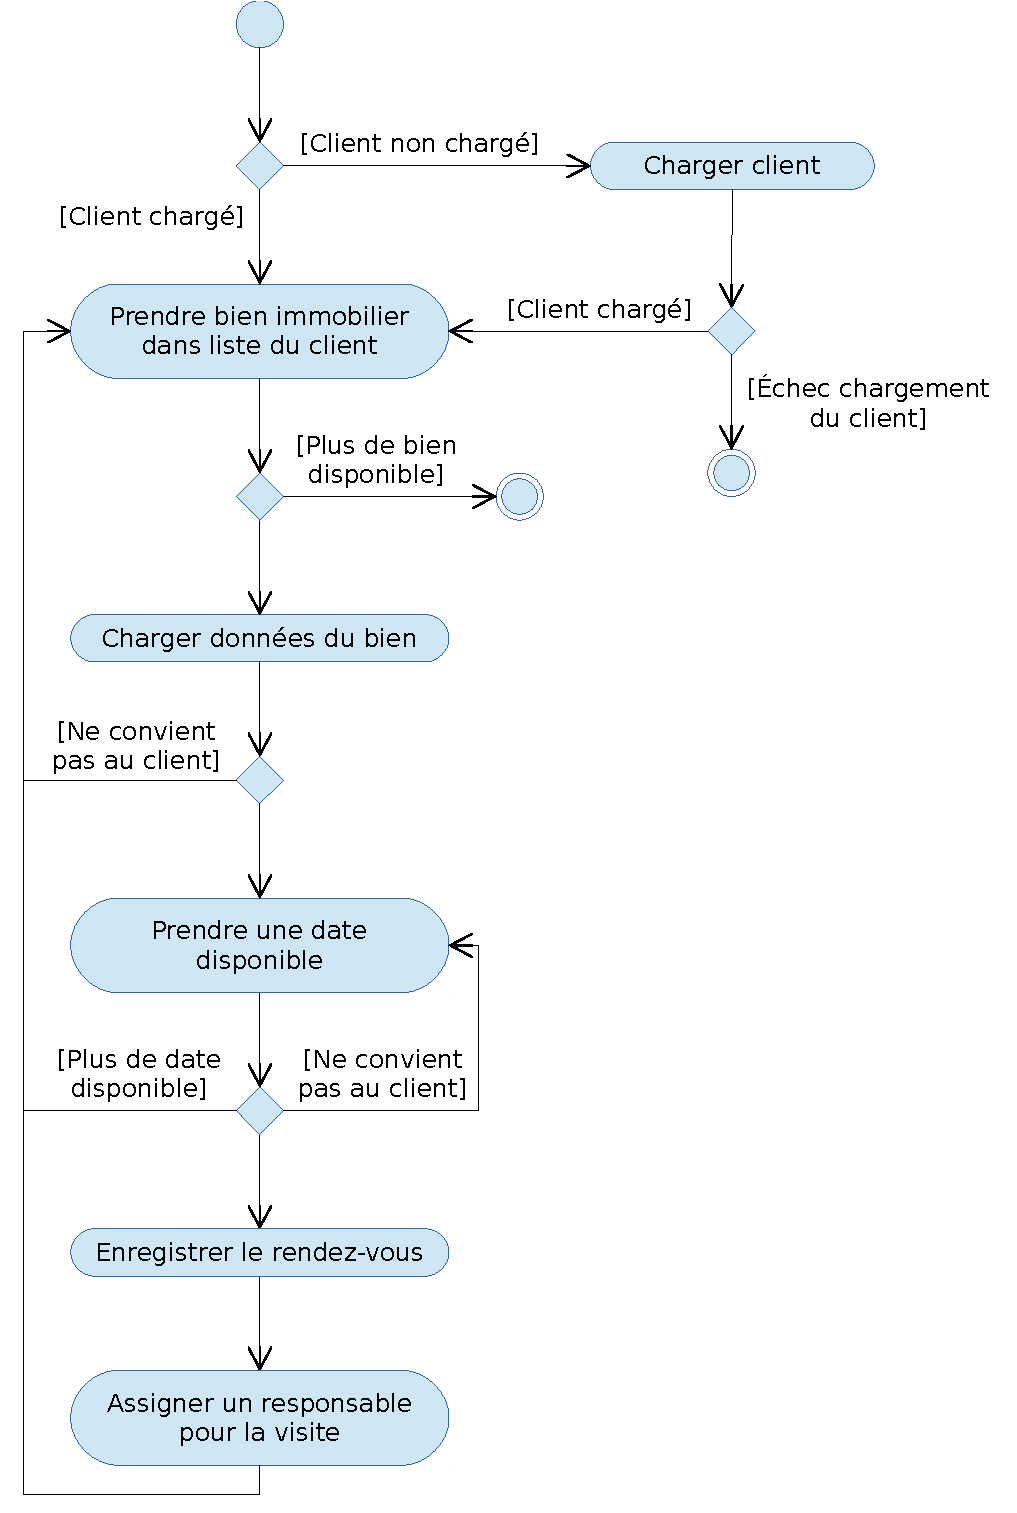
\includegraphics[scale=0.67]{IMG/ad}
  \caption{Diagramme d'activité}
  \label{img_ad}
\end{figure}

La figure \refpage{img_ad} illustre le diagramme d'activité du cas d'utilisation \selectedusecase{}.

\section{Rapport}

Ce diagramme est basé sur le scénario du cas d'utilisation \selectedusecase{}. Il sert à modéliser les différentes actions qui seront effectuées pour réaliser ce cas d'utilisation dans son ensemble. L'acteur \og{}employé\fg{}, qui est le seul acteur du système, interviendra dans ce cas d'utilisation.

Si l'employé est déjà en train de traité des informations concernant le client en cours, son dossier avec la liste des propriétés proposées sera déjà disponible au début de cette activité. Sinon, l'employé devra charger ce dossier dans le système.

L'employé va parcourir la liste des propriétés proposées au client. Pour chaque propriété, les données détaillées de celle-ci seront chargées. Le client pourra émettre un avis. Si le client marque un intérêt pour la propriété, l'employé va retenir le bien. Sinon, il va le marquer comme non intéressant.

Ensuite, pour chaque propriété retenue par le client, les dates des visites déjà planifiées seront affichées. L'employé pourra déterminer, sur base des dates fournies, une date de visite.

Une fois qu'une date a été déterminée avec le client, un rendez-vous sera sera organisé pour la visite. Un employé du service des visites sera désigné pour accompagner le client.

À la fin de cette activité, nous aurons généré une liste de rendez-vous pour les visites du bien par le client.